%% Hello emacs, this is -*- latex -*-
\typeout{ ====================================================================}
\typeout{ This is file neuralringer.tex, created at 27-Aug-2005 }
\typeout{ Maintained by Andre Anjos <Andre.dos.Anjos@cern.ch> }
\typeout{ ====================================================================}

\chapter{\eng{NeuralRinger}: Projeto e implementação}
\label{ap:framework}

O projeto do \eng{NeuralRinger} está dividido em quatro sub-pacotes que
executam funções bem-definidas para o interfaceamento, configuração e execução
de redes neurais. A Figura~\ref{fig:nr-packages} contém um diagrama UML (do
inglês, \eng{Unified Modelling Language}, \cite{booch}) nomeando e
mostrando a relação de dependência entre estes pacotes.

\begin{figure}
\begin{center}
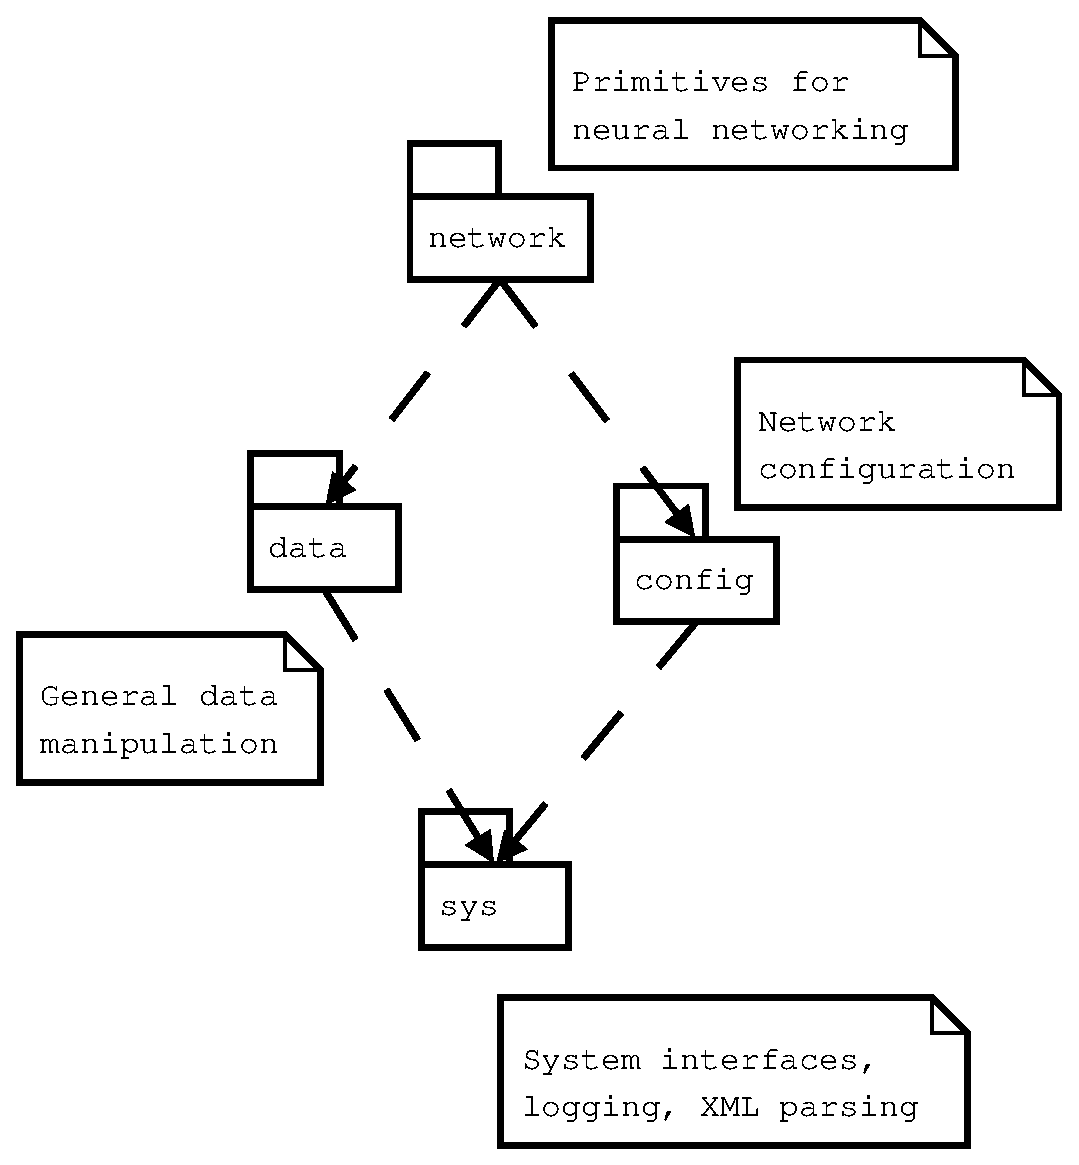
\includegraphics[scale=0.5]{nr-packages}
\end{center}
\caption{Diagrama de blocos mostrando a relação entre os pacotes do
\eng{NeuralRinger}.}
\label{fig:nr-packages}
\end{figure}

\paragraph{\texttt{SYS}:} O sub-pacote \texttt{sys} está abaixo na cadeia de
dependências e não depende de nenhum outro. Este pacote inclui ferramentas
para a manipulação de arquivos no formato XML (do inglês
\eng{eXtensible Markup Language}, \cite{xml}) e um sistema básico para
o relatório de erros. A escolha da linguagem XML, como formato de troca de
dados e valores de configuração, vem da grande quantidade de interpretadores
(\eng{parsers}) disponíveis livremente na \eng{Internet}, já que é um padrão
bastante difundido. O suporte a XML disponível atualmente inclui, mas não se
limita a, verificações de sintaxe automatizadas (via
\eng{XML schemas}) e transformações para que se adicione informação ou seja
possível a visualização, de forma adequada, do conteúdo de uma base de dados
XML.

A Figura~\ref{fig:sys-uml} traz uma visão geral dos componentes e seu
relacionamento dentro deste pacote. Na parte central do diagrama, encontra-se o
tipo \texttt{Reporter} que define uma interface para o relatório de
erros. Objetos deste tipo contêm uma implementação específica do sistema de
relatório de erros. Inicialmente, somente a implementação baseada em
arquivos-padrão tais como \texttt{std::cout} e \texttt{std::cerr}
\cite{web:gcc-stl} foi desenvolvida. 

À direita observa-se a modelagem para o sistema de interpretadores XML. Uma
interface (abstrata) é utilizada como base para implementações específicas
baseadas em interpretadores habitualmente encontrados nos sistemas
operacionais correntes. Especificamente, implementações para o sistema Xerces
C++ \cite{xerces-c}, do grupo Apache e libxml2 \cite{libxml2}, do grupo GNOME,
estão presentes na implementação atual. O interpretador XML utiliza-se do
sistema de relatório de erros para relatar problemas na leitura ou escrita de
arquivos de forma unificada. Uma caixa de ferramentas baseada no tipo abstrato
\texttt{XMLProcessor} provê um conjunto de primitivas para facilitar a escrita
e a leitura de parâmetros e trechos de texto. No evento de erros fatais, uma
exceção baseada no tipo \texttt{Exception} será lançada pela parte afetada do
código.

\begin{figure}
\begin{center}
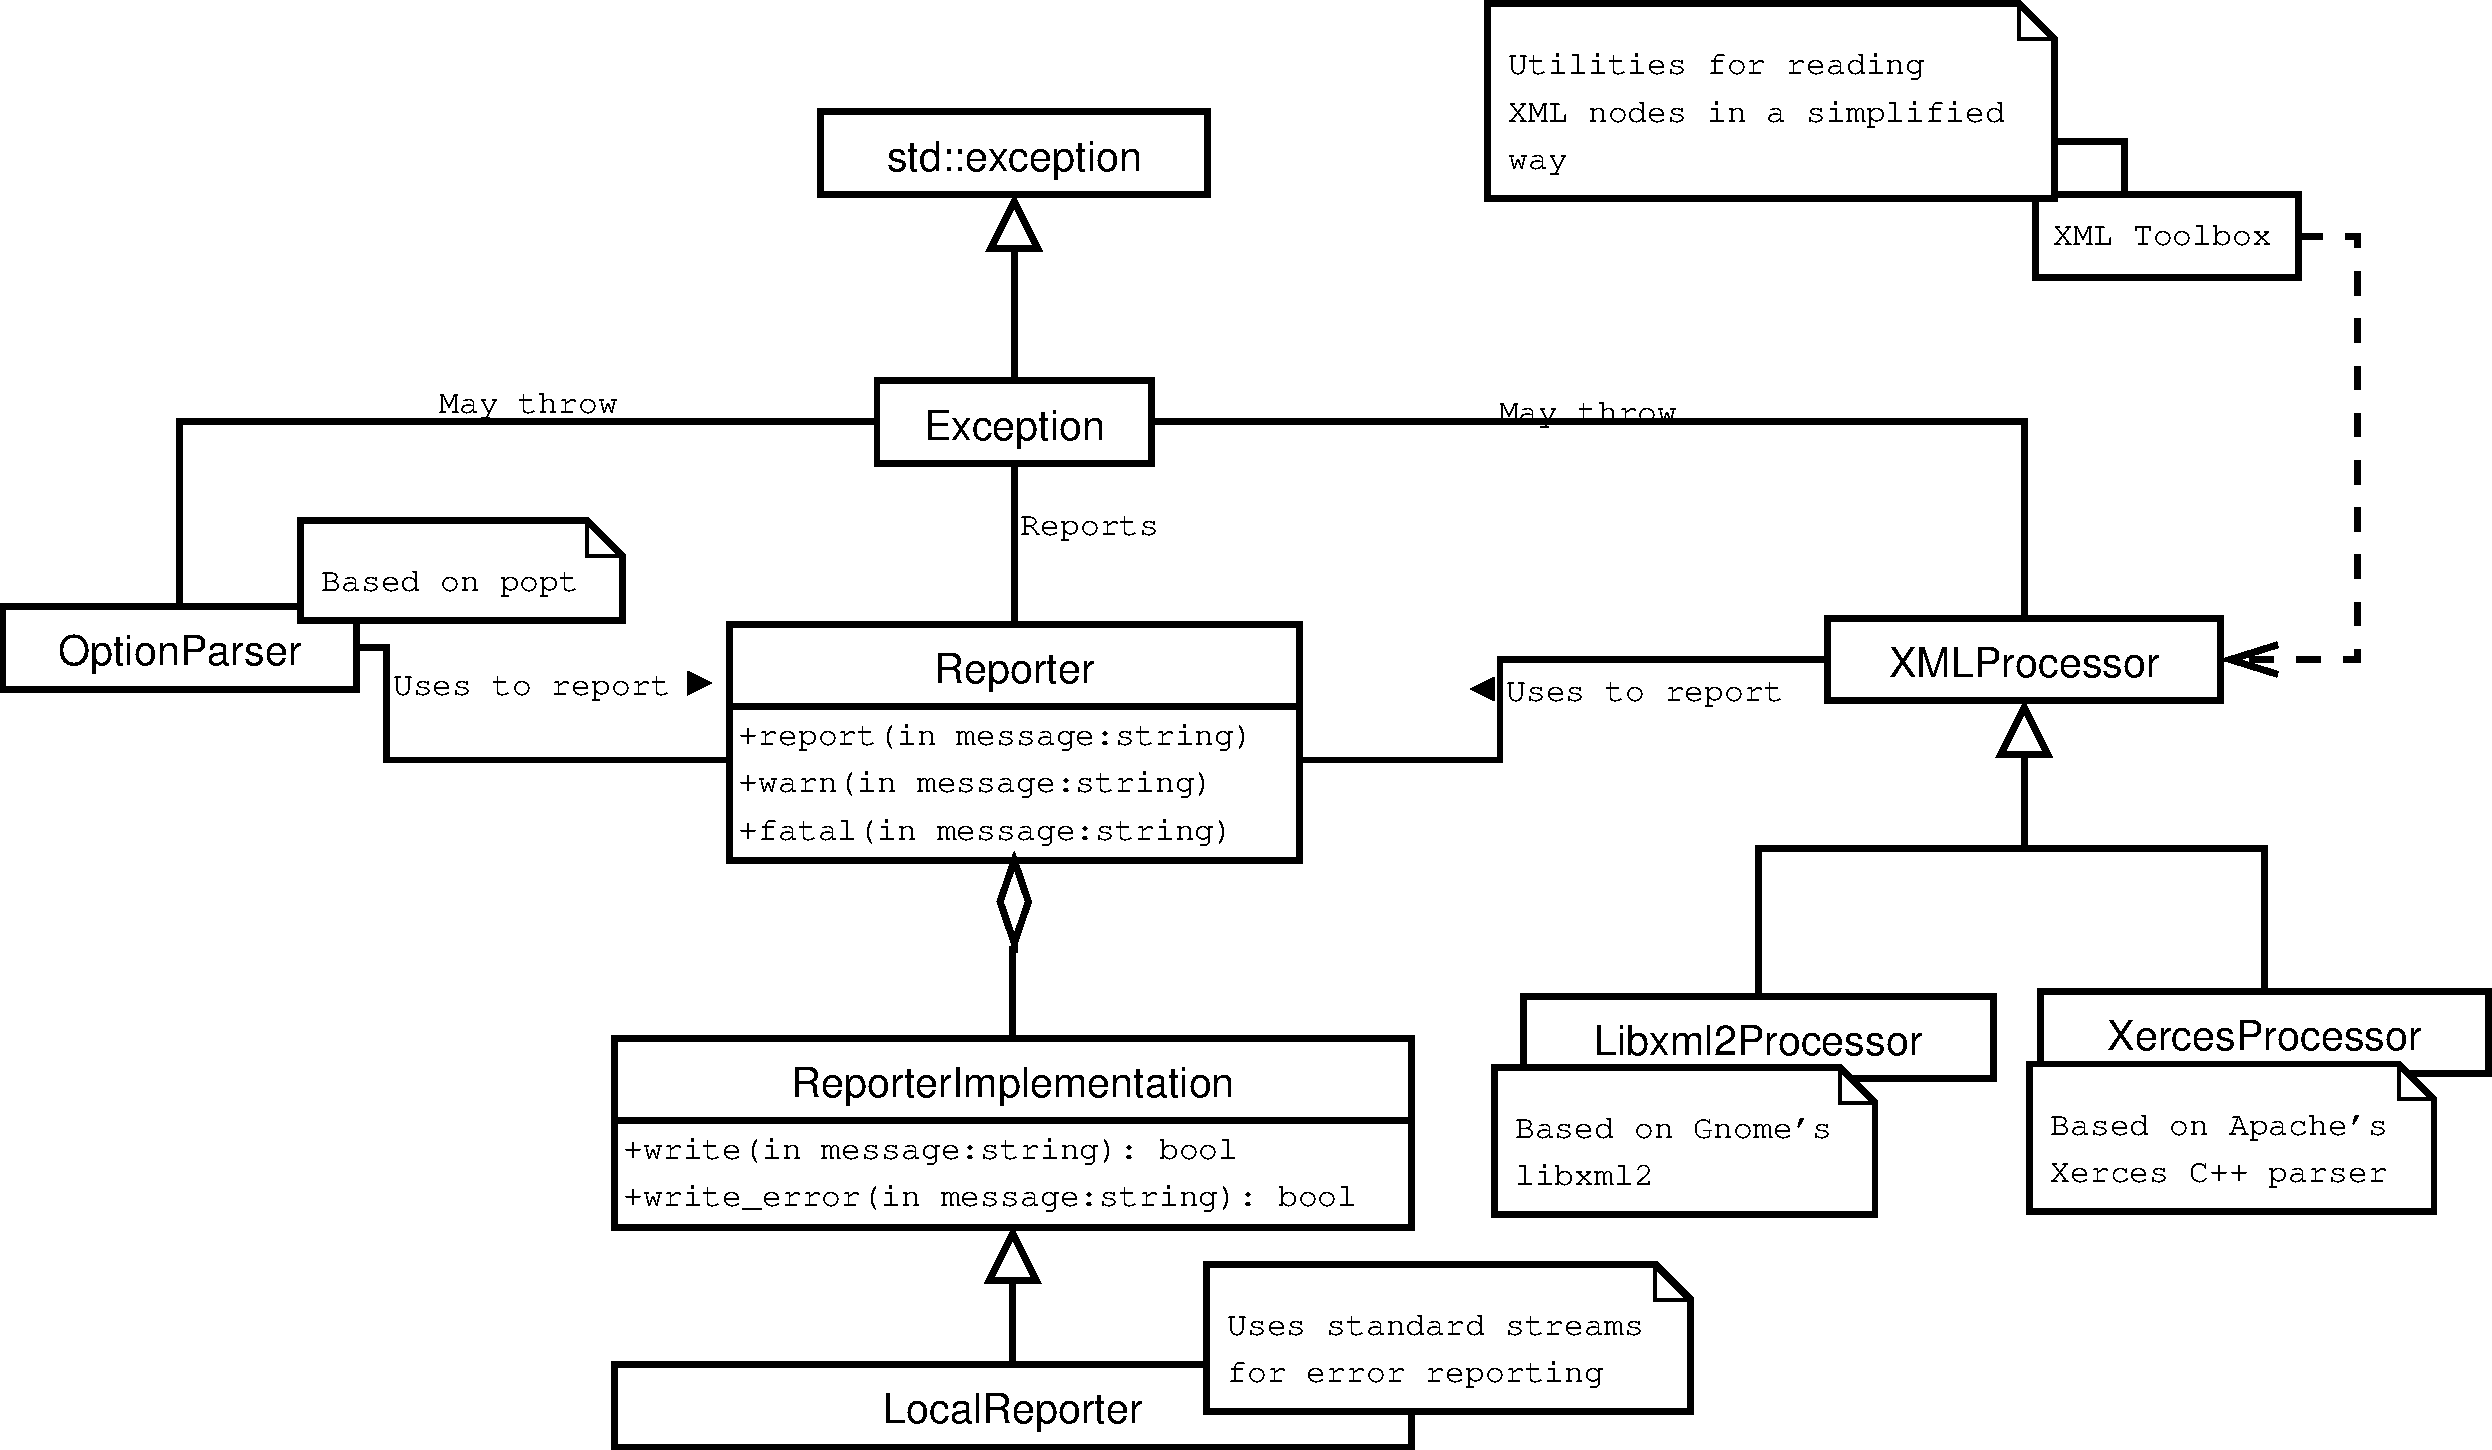
\includegraphics[scale=0.34]{sys-uml}
\end{center}
\caption{Diagrama UML mostrando as relações dos componentes do pacote
\texttt{sys}.}
\label{fig:sys-uml}
\end{figure}

O pacote \texttt{sys} também fornece um sistema para a interpretação de opções
de linha de comando, baseado no interpretador \texttt{popt}. Este tipo imbute
um sistema de atribuição automática e verificação de valores, conectando as
opções na linha de comando diretamente com o contexto onde as opções serão
utilizadas dentro do programa. Seguindo a filosofia dos interpretadores XML,
este tipo também faz uso do sistema central de relatório de erros para
informar problemas ao usuário e poderá, no caso de problemas sérios, também
lançar exceções de operação.

\paragraph{\texttt{DATA}:} O pacote \texttt{data} contém as primitivas para a
manipulação dos dados, prévia e posteriormente ao processamento neural. Este
sub-sistema utiliza-se das primitivas definidas no pacote \texttt{sys} para
executar a reportagem de erros, lançamento de exceções ou a leitura de
arquivos XML. A implementação das primitivas neste pacote utiliza elementos
otimizados da biblioteca GSL (\eng{GNU Scientific Library}, \cite{gsl}) para a
manipulação de valores contidos em matrizes e vetores. A
Figura~\ref{fig:data-uml} mostra um diagrama indicando a relação das classes
dentro do pacote \texttt{data}.

\begin{figure}
\begin{center}
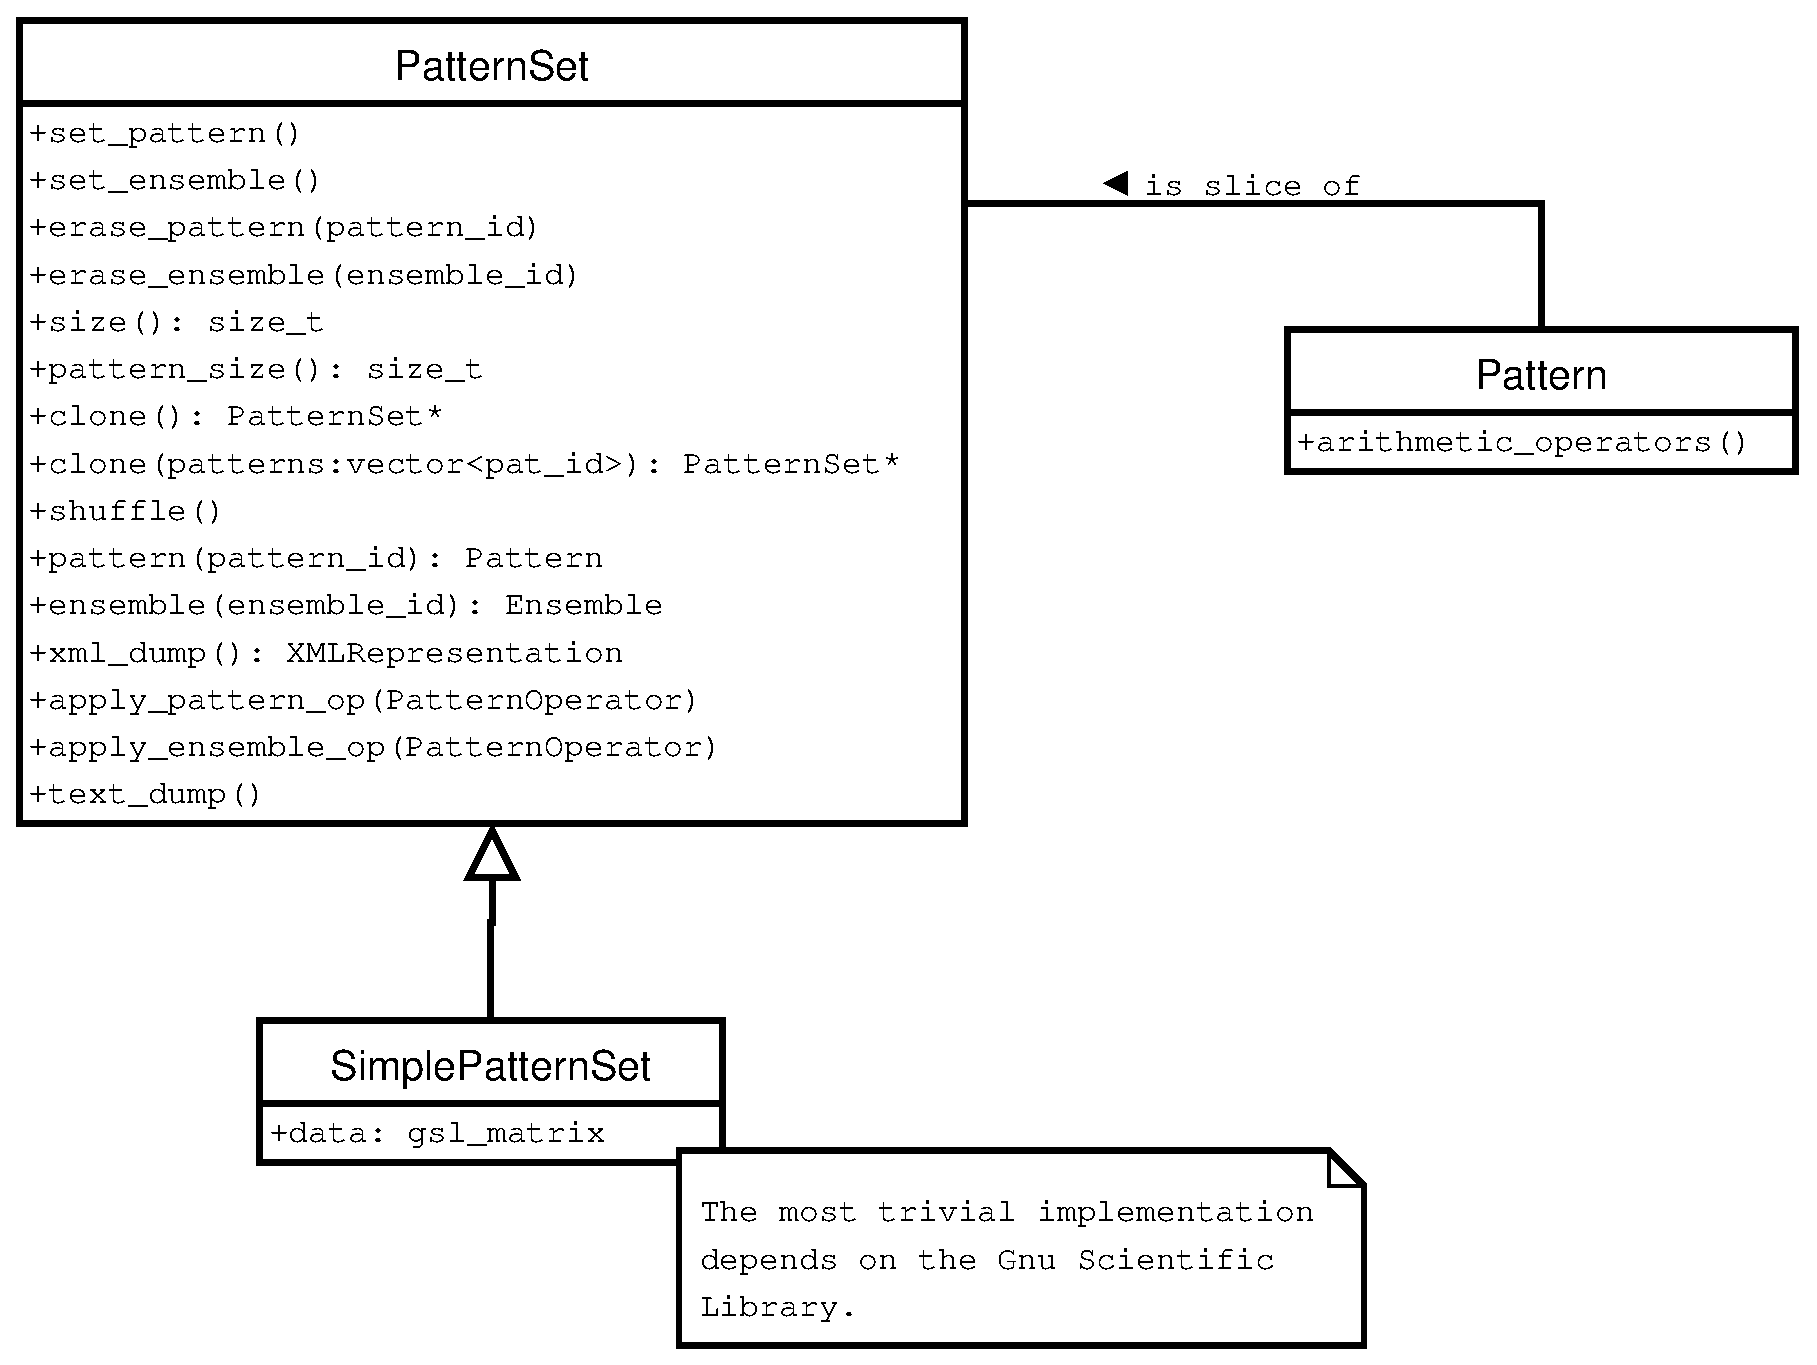
\includegraphics[scale=0.3]{data-uml}
\end{center}
\caption{Diagrama UML mostrando as relações dos componentes do pacote
\texttt{data}.}
\label{fig:data-uml}
\end{figure}

O elemento central deste pacote chama-se \texttt{PatternSet}. Ele representa
um conjunto de vetores ou padrões formando uma matriz de dados. Esta matriz é
representada internamente por um objeto tipo matriz GSL
(\texttt{gsl$\_$matrix}). Para o armazenamento dos dados, utilizou-se a
seguinte estratégia: cada evento do fenômeno observado será guardado em uma
linha da matriz. Neste caso, cada coluna representará uma característica (ou
\eng{Feature} no inglês) do dado. A biblioteca GSL permite acesso rápido tanto
aos padrões (linhas) como características (colunas) da matriz de dados. 

Baseando-se nas primitivas de acesso ao tipo matriz GSL, a classe base
\texttt{PatternSet} desenvolve mé\-todos tí\-picos utilizados durante a
manipulação dos dados, tais como acesso simplificado, leitura e escrita em
disco, mistura dos padrões, manipulação de campos específicos e cópia. O
formato de escrita em disco escolhido utiliza o padrão XML. O banco de dados
básico contém um cabeçalho com as informações do autor e dos dados, indicando
a data de criação e a última atualização. Dentro do arquivo, os dados podem
ser dividos em classes. Cada classe é dividida por sua vez em padrões, que
contêm um número opcional de atributos.

Para o caso específico do processamento de dados de RoIs, uma classe é
derivada da implementação de base de um \texttt{PatternSet}, chamada
\texttt{RoIPatternSet}. Esta classe implementa, adicionalmente à classe de
base, métodos para a salvaguarda, leitura e manipulação de campos
especificamente relacionados a uma RoI, assim como os identificadores do
primeiro nível de filtragem e os valores das coordenadas $\eta$ e $\phi$.
Desta forma, é possível correlacionar os resultados obtidos com outros testes
ou com relação ao posicionamento da região de interesse. Exemplos de conjuntos
de padrões são elétrons ou jatos.

Uma coleção de um ou mais conjuntos de padrões é chamada \texttt{Database}, ou
banco de dados. Um banco de dados reúne os diferentes conjuntos de padrões que
se deseja processar através de um mapa. Para cada conjunto de padrões, o
usuário pode atribuir um nome, mapeando os dados propriamente ditos a um valor
legível por uma outra pessoa. Usando um objeto da classe \texttt{Database}, é
possível manipular os conjuntos de padrões de uma forma unificada, por
exemplo, quando deseja-se extrair a média ou desvio padrão global dos
conjuntos de padrões de um problema.

Operadores (\texttt{PatternOperator}s no diagrama), são elementos que podem
modificar um padrão e são usados para extrair a média, variância ou aplicar
normalizações segundo diferentes critérios nos dados disponíveis. Na figura,
mostra-se o mais relevante dos operadores na biblioteca, chamado
\eng{NormalizationOperator}, que é inicializado a partir de uma base de dados
e pode, quando aplicado a um padrão, remover a média e desvio padrão da base
de dados. Este operador é utilizado em todos os testes neste trabalho como
forma de normalização dos dados de entrada de classificadores LMS ou Redes
Neurais. Quando um operator é aplicado a um padrão, primitivas da biblioteca
GSL são utilizadas para que a eficiência do processo seja maximizada.

\paragraph{\texttt{NETWORK}:} Este pacote contém a definição de
neurônios, sinapses e redes formadas a partir destes elementos. A
Figura~\ref{fig:network-uml} apresenta um diagrama UML dos tipos neste
sub-sistema. No topo deste diagrama está o tipo \texttt{Network} (Rede), que
representa, de forma abstrata, um conjunto de neurônios (tipo \texttt{Neuron})
interconectados via objetos do tipo sinapse (tipo \texttt{Synapse}). Uma rede
pode ser executada utilizando-se um dos métodos \texttt{run()} e treinada
usando-se uma das variantes de \texttt{train()}. De fato, objetos do tipo
\texttt{Network} não contêm nenhuma informação direta sobre a topologia da
rede que executam, funcionando apenas como agentes delegadores de
responsabilidade. O sistema funciona da seguinte forma:

\begin{figure}
\begin{center}
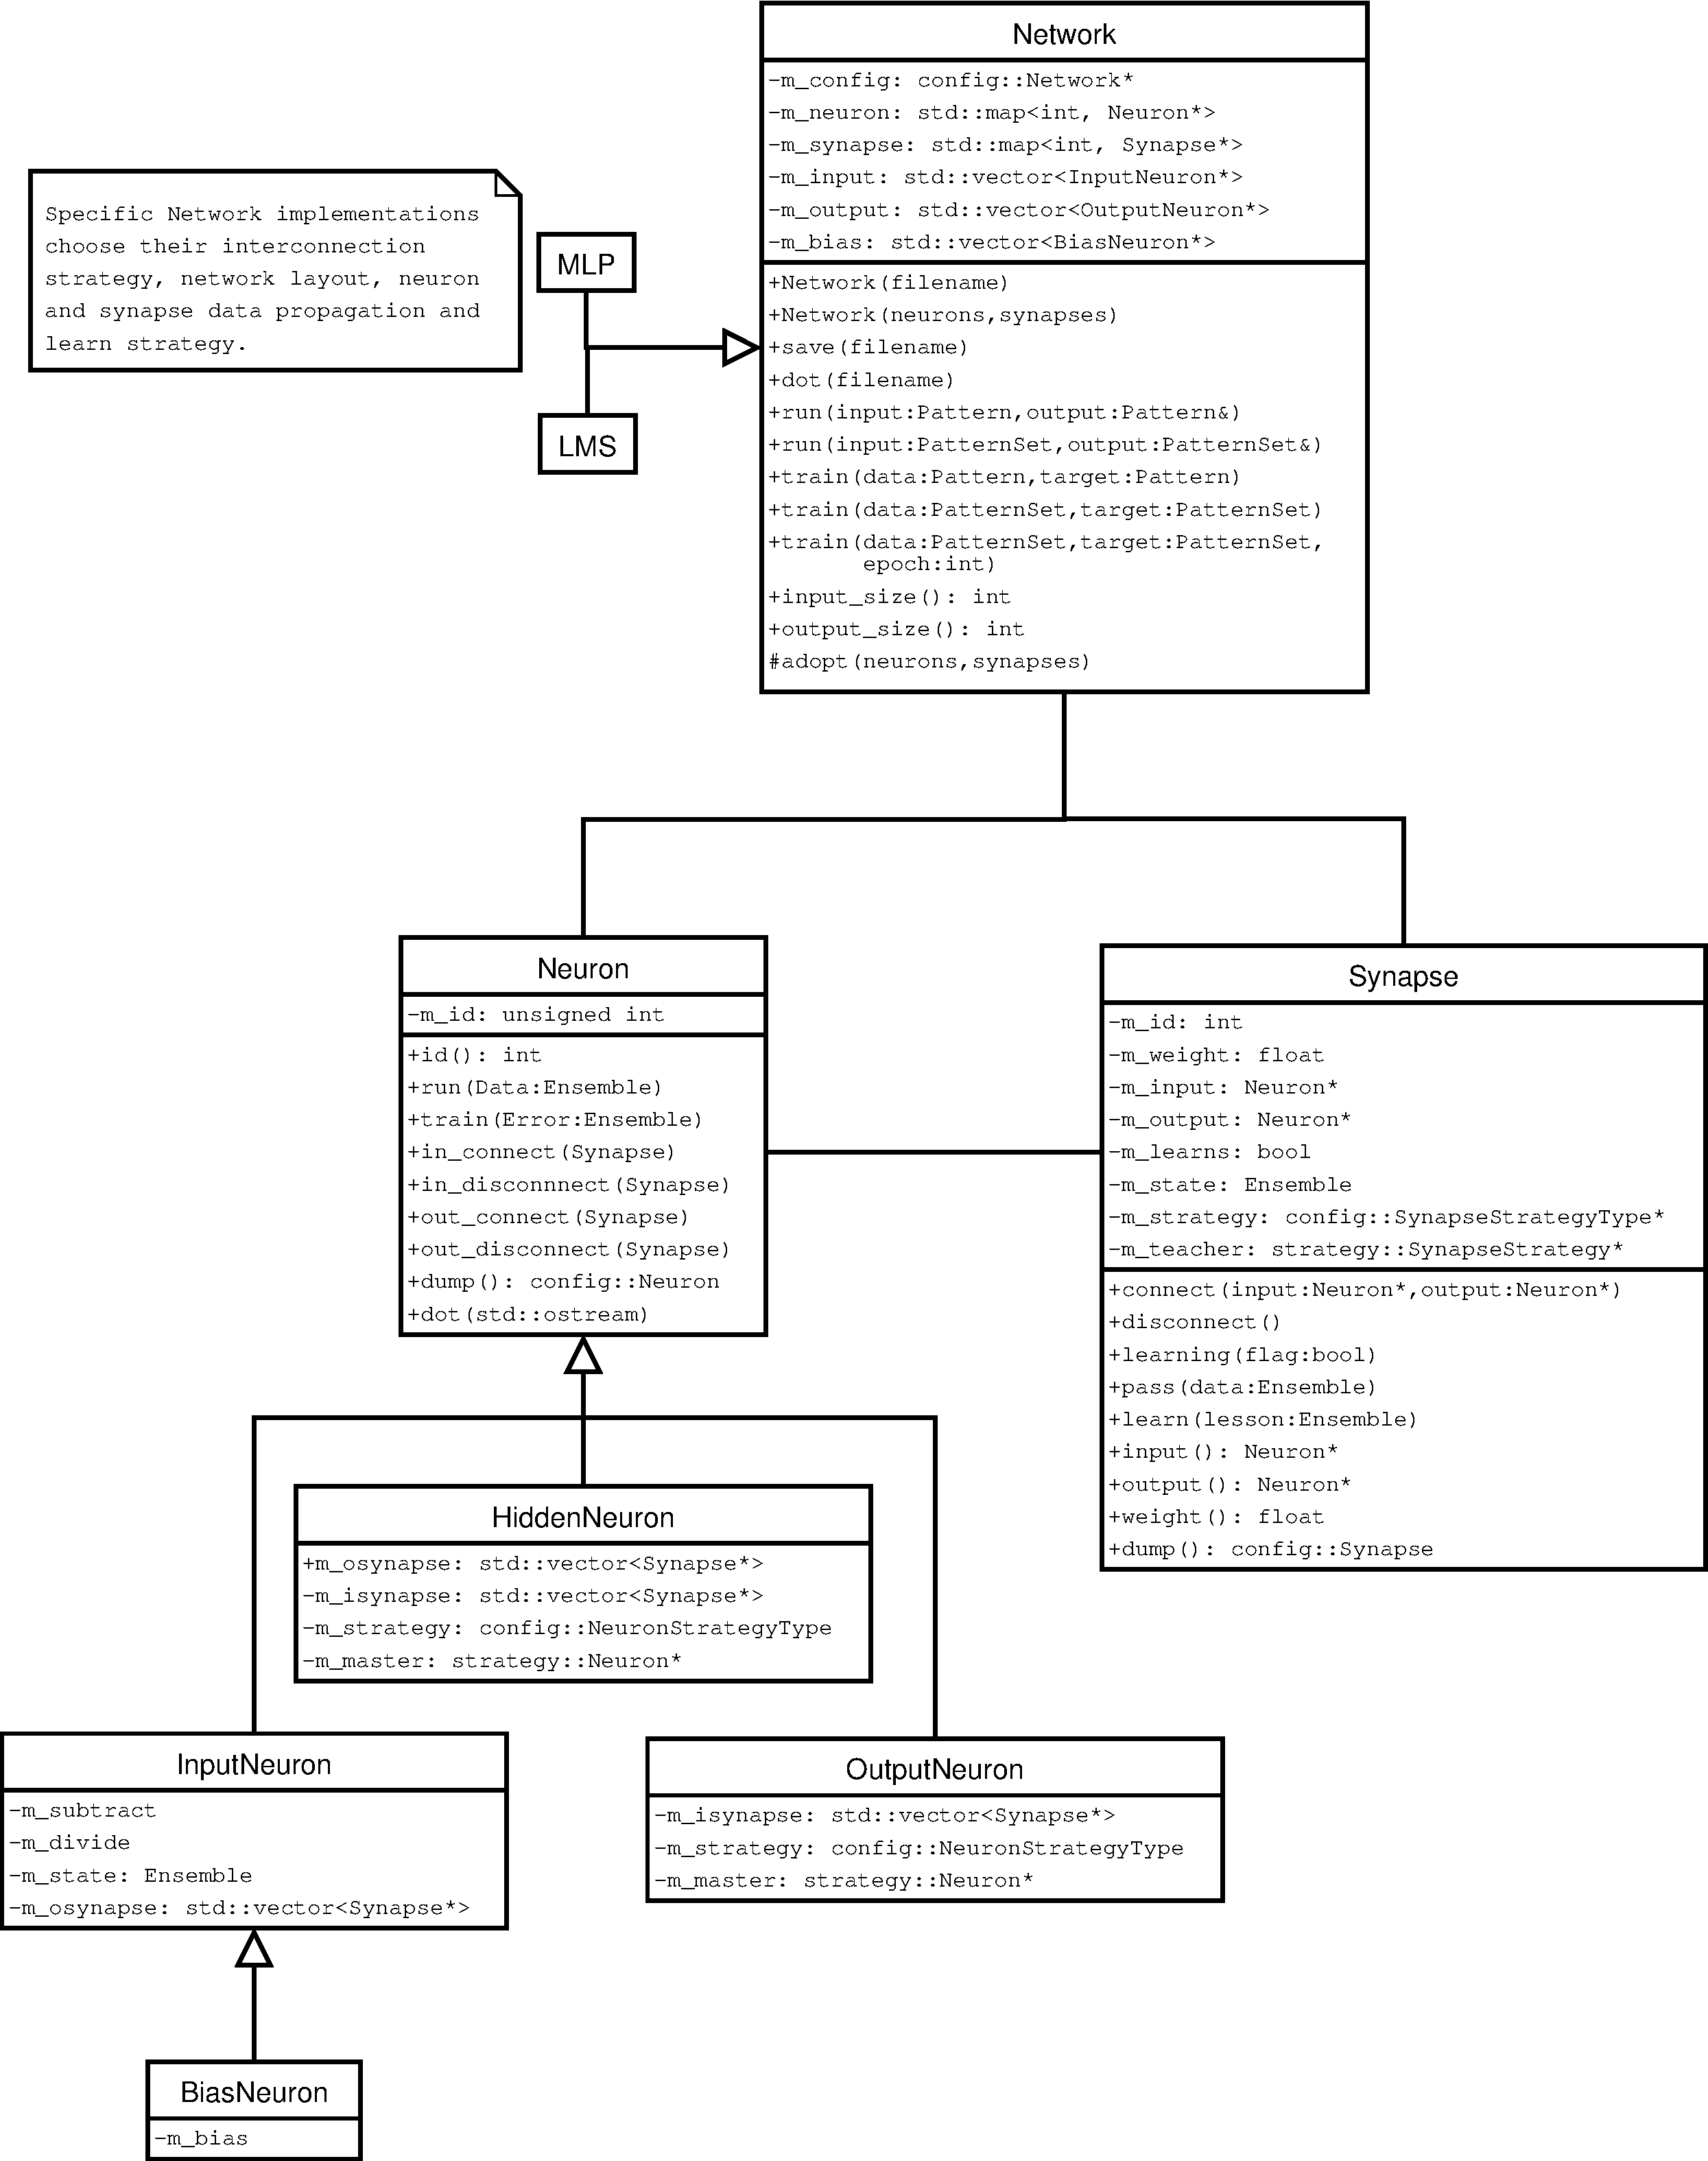
\includegraphics[scale=0.35]{network-uml}
\end{center}
\caption{Diagrama UML mostrando as relações dos componentes do pacote
\texttt{network}.}
\label{fig:network-uml}
\end{figure}

\begin{itemize}
\item \textbf{Para executar a rede}: Neste modo, o usuário irá iniciar o
processo aplicando à entrada da rede um padrão ou conjunto de padrões. O
objeto do tipo \texttt{Network} irá, então, para cada coluna da matriz de dados
de entrada, chamar o método \texttt{run()} dos neurônios de entrada,
correlacionando os dados do usuário com as posições relativas do neurônio da
camada de entrada. Opcionalmente, se existirem neurônios de polarização
(\texttt{BiasNeuron}s), o mesmo será feito para cada um destes neurônios. Cada
neurônio de entrada e polarização é responsável por propagar seu sinal aos
neurônios ao qual está conectado, através das sinapses (objetos do tipo
\texttt{Synapse}). As sinapses irão multiplicar o valor de suas entradas pelo
seu próprio peso e propagar o sinal ao neurônio destino. Este último, após
receber todas as entradas relativas às sinapses que estão conectadas a si,
executará o mesmo procedimento até que o sinal chegue ao neurônio de saída da
rede.

\item \textbf{Para treinar a rede}: O sistema de treinamento funciona de 
modo equivalente. Uma vez calculado o sinal de erro, ou a \textit{lição} a
partir da técnica que convier, este sinal é injetado ao neurônio de saída, que
retropropagará o sinal até o neurônio de entrada.
\end{itemize}

Os tipos de neurônio são divididos nas seguintes classes:

\begin{itemize}
\item Entrada (\texttt{InputNeuron}): são neurônios que recebem a entrada
da rede, opcionalmente aplicando um fator de normalização aos dados e
propagando o sinal para neurônios escondidos ou de saída. Como estão no início
da rede, estes neurônios não podem retropropagar sinais recebidos em suas
saídas para fins de treinamento. Uma vez que atingem estes neurônios, os
sinais de erro retropropagados são apagados da memória e o passo de
treinamento é considerado como executado;

\item Polarização (\texttt{BiasNeuron}): este tipo herda suas 
caracte\-rís\-ticas da classe \texttt{In\-put\-Neuron}, mas não permite que o
usu\-á\-rio defina uma entrada arbitrária que será propagada a rede. No lugar,
é possível definir um valor fixo (normalmente $+1$), que é alimentado, via
sinapses de conexão, aos neurônios de saída ou escondidos;

\item Escondido (\texttt{HiddenNeuron}): são neurônios que estão entre os
neurônios de entrada e/ou polarização, conectando a entrada à saída. São
opcionais, já que é possível desenvolver redes sem neurônios desta
classe. Neurônios escondidos transmitem os dados recebidos em suas entradas a
seus neurônios de saída, aplicando uma operação de soma aos valores de
entrada, seguida, opcionalmente de uma função de ativação configurável;

\item Saída (\texttt{OutputNeuron}): são os neurônios que estão na saída da
rede. Seus valores constituem a saída do sistema neural. Assim como os
neurônios escondidos, podem aplicar uma função de ativação ao campo induzido
produzido somando-se os dados de entrada.
\end{itemize}

A execução da rede e treinamento das sinapses é regido por dois parâmetros que
estão atrelados a estes elementos: as estratégias. Estratégias para neurônios
(objetos da classe \texttt{NeuronStrategy}) definem de que forma os neurônios
propagaram os sinais de erro quando são injetados na saída rede, para correção
dos valores sinápticos. No momento, há somente um tipo de estratégia possível:
a retropropagação de erros. Três funções de ativação estão implementadas: a
função linear (utilizada para redes tipo LMS), a função logística
simplificada, definida na Equação~(\ref{eq:logf}) e a função tangente
hiperbólica, definida na Equação~(\ref{eq:tanh}).

Métodos para salvaguardar e restaurar uma rede a partir de um arquivo es\-tão
implementados. A salvaguarda é implementada através de um processo iterativo
de delegação de responsabilidades, em que cada neurônio e sinapse envolvidos na
rede se auto-descrevem no arquivo de saída. O formato escolhido é XML, uma vez
que as bibliotecas de base do pacote \texttt{sys} já implementam as primitivas
de leitura e escrita neste formato. Um segundo método (chamado \texttt{dot()})
está disponível para objetos do tipo rede. Este método implementa a
escrita em disco de uma descrição da rede no formato \texttt{dot}
\cite{graphviz}, que permite a visualização dos pesos e interconexões da rede
de forma gráfica. Exemplos de uma rede LMS e uma rede MLP encontram-se nas
Figuras~\ref{fig:lms-dot-example} e ~\ref{fig:mlp-dot-example},
respectivamente. As caixas na parte esquerda da figura representam o fator de
normalização aplicado às entradas. Os círculos à esquerda, seguindo o caminho
de propagação do sinal representam os neurônios de entrada. Cada neurônio
possui uma numeração única, que o distingue dos outros. Este número
corresponde ao identificador usado dentro das aplicações do
\eng{NeuralRinger}. 

Neurônios escondidos e aqueles pertencentes à camada de saída são
representados por uma caixa com as bordas arredondadas. Nesta caixa, o
identificador do neurônio está representado na parte superior esquerda. Na
parte inferior desta região, abaixo do identificador, um sinal de adição ($+$)
indica que as entradas deste neurônio serão somadas antes da aplicação da
função de ativação, definida na parte esquerda. Nós de polarização são
mostrados junto ao neurônio a que estão conectados. Os diversos neurônios são
conectados por retas que apontam na direção da propagação do sinal de entrada
da rede. A saída da rede é mostrada usando-se um círculo e localizada na
extrema direita da figura. O número dentro deste círculo corresponde ao
identificador do neurônio de saída e casa com o número indicado no retângulo que
precede o círculo.

\begin{figure}
\begin{center}
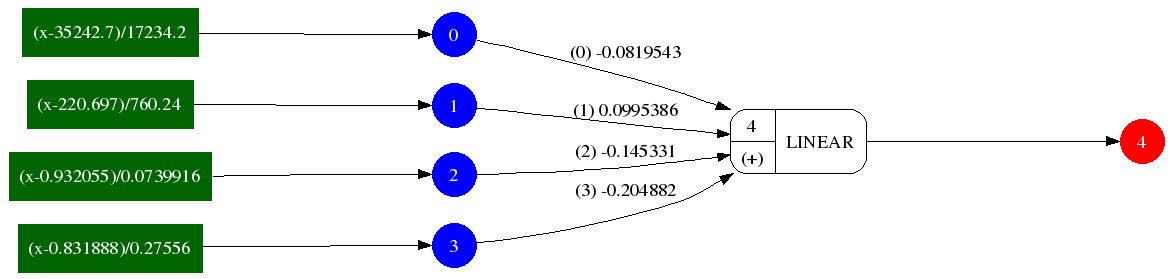
\includegraphics[scale=0.35]{lms-best2}
\end{center}
\caption{Exemplo de um gráfico de fluxo produzido pelo método \texttt{dot()}
para uma rede LMS, tal qual utilizada para os testes na
Seção~\ref{sec:linear}.}
\label{fig:lms-dot-example}
\end{figure}

\begin{figure}
\begin{center}
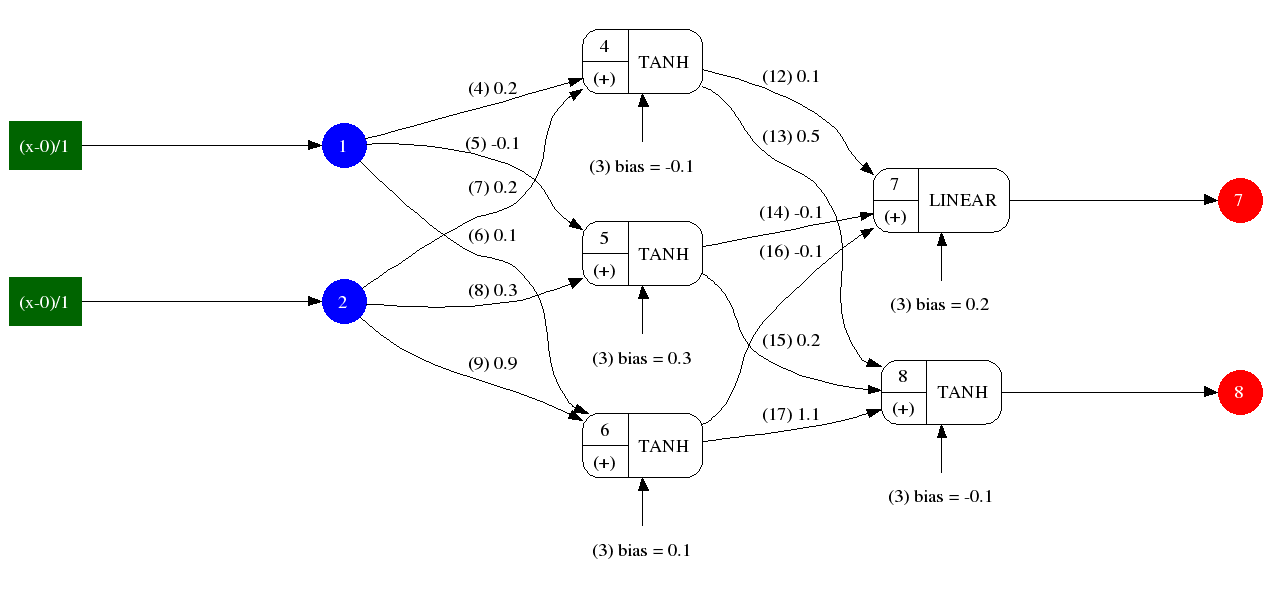
\includegraphics[scale=0.32]{mlp-caloba.png}
\end{center}
\caption{Exemplo de uma gráfico de fluxo produzido pelo método \texttt{dot()}
para uma rede MLP.}
\label{fig:mlp-dot-example}
\end{figure}

\paragraph{\texttt{CONFIG}:} Este pacote implementa a leitura e a escrita de
parâmetros de redes a um arquivo XML. É um pacote que depende da
infraestrutura provida pelo pacote \texttt{sys} e provê suporte à
configuração das redes definidas no pacote \texttt{network}.

\paragraph{Outros pacotes:} O \eng{NeuralRinger} contém, ainda, 3 outros
sub-projetos que apoiam sua funcionalidade:

\begin{itemize}
\item \texttt{lvl1}: contém um simulador simplificado da filtragem baseada em
calorimetria executada no LVL1. Este pacote pode ser utilizado para filtrar,
dentre as regiões de interesse disponíveis, aquelas que seriam aprovadas pelo
LVL1. Ele pode ser usado no lugar de uma simulação completa do Athena para
separar dados para uma análise menos criteriosa. Para o filtro de referência,
é preferível que o usuário utilize o programa Athena;

\item \texttt{roiformat}: define o formato de intercâmbio entre o sistema de
calorimetria implementado no Athena e o \eng{NeuralRinger}, possibilitando que
os dados disponíveis no primeiro possam ser facilmente escritos em disco e
lidos por versões do \eng{NeuralRinger} não acompladas ao Athena. Isso
normalmente diminui o tempo de desenvolvimento e teste, e é aconselhável;

\item \texttt{rbuild}: este pacote contém primitivas para a construções de
anéis baseados nos dados brutos das RoI disponíveis. Este método de deteção é
uma alternativa mais eficaz ao processamento utilizando as características
definidas pelo T2Calo. Este sistema será introduzido mais adiante.
\end{itemize}

\subsubsection{Aplicações:}

Um conjunto de aplicativos foi escrito utilizando o sistema de pacotes
definido na seção anterior. Estes aplicativos podem ser executados
independentemente do sistema Athena, o que simplifica o desenvolvimento e
treinamento das redes neurais, assim como a depuração de eventuais problemas
no código. Estes são os programas disponíveis:

\begin{itemize}

\item \textbf{eta-filter}: Este programa pode sub-dividir uma base de dados
contendo RoIs, de forma a classificar os dados por segmentos em $\eta$. O
programa é iniciado com um arquivo contendo as RoIs no formato XML padrão e
com um valor para $|\Delta_\eta|$. Para cada sub-intervalo de tamanho
$|\Delta_\eta|$ dentro do intervalo $[-2,5, +2,5[$, um arquivo de dados é
gerado. Estes arquivos conterão dados para RoIs nos respectivos intervalos em
$\eta$. O processamento leva em consideração a localização da RoI determinada
pelo LVL1, que está disponível nas bases de dado XML;

\item \textbf{getroi}: Separa RoIs de uma base de dados no formato
\texttt{roiformat} para inspeção por um programa externo;

\item \textbf{lms-train}: Implementa um sistema completo de treinamento 
de uma rede LMS. O sistema é configurável quanto aos parâmetros de
treinamento, permitindo a especificação da taxa de treinamento, tamanho da
época, critério de parada, tempo de parada abrupta e os nomes dos arquivos de
entrada e saída;

\item \textbf{lvl1-filter}: Este programa implementa um filtro baseado em uma
simulação simplificada do LVL1. Ele pode ser utilizado para filtrar, dentre as
regiões de interesse disponíveis, aquelas que seriam aprovadas pelo LVL1. O
usuário poderá especificar os diversos limites de corte para a filtragem do
primeiro nível:

\begin{itemize}
\item Limite hadrônico;
\item Limite eletromagnético e
\item Isolamento eletromagnético;
\end{itemize}

\item \textbf{merge}: Este programa pode aglutinar múltiplas bases de dados
XML em um único arquivo de saída; 

\item \textbf{mlp-relevance}: Este programa avalia a relevância das
características de entrada de uma rede (LMS ou MLP), tanto considerando-se o
valor MSE quanto o produto SP originais da rede;

\item \textbf{mlp-run}: Roda uma rede (LMS ou MLP) e escreve uma base de dados
de saída com os resultados;

\item \textbf{mlp-train}: Implementa um sistema completo de treinamento de 
uma rede MLP. De forma análoga ao programa \texttt{lms-train}, esta aplicação
é configurável quanto aos parâmetros de treinamento, permitindo a
especificação da taxa de treinamento, tamanho da época, critério de parada,
tempo de parada abrupta e os nomes dos arquivos de entrada e saída;

\item \textbf{relevance-filter}: Este programa pode remover uma ou mais
colunas de uma matriz de dados, baseando-se na análise da relevância e um
parâmetro de corte. Com este programa também é possível reduzir o espaço de
entrada de um discriminador, minimizando as perdas na classificação, como será
mostrado mais à frente;

\item \textbf{ringer}: Este programa pode calcular, levando-se em consideração
um padrão de normalização, os anéis de energia que serão utilizados nesse
trabalho. A saída deste programa é uma base de dados no formato XML padrão do
\eng{NeuralRinger};

\item \textbf{ringer-run}: Este programa executa a extração e a discriminação
de elétrons e jatos baseado na técnica do anelamento, descrita no
Capítulo~\ref{chap:neural}. Ele pode ser utilizado para o cálculo do
desempenho do algoritmo de filtragem \eng{offline} e permite uma otimização da
execução antes da implementação no ambiente Athena;

\item \textbf{xml2dot}: Escreve a representação de uma rede no formato
\texttt{dot} para que seja possível a visualização tal qual no exemplo das
Figuras~\ref{fig:lms-dot-example} e \ref{fig:mlp-dot-example};

\item \textbf{xml2text}: Este programa converte uma base de dados no formato
XML padrão do \eng{NeuralRinger} em uma representação no formato texto, que
pode ser lido por programas que não suportem XML.
\end{itemize}

Cada um dos programas responde ao comando \texttt{--help}, que imprime na tela
o conjunto de opções e valores padrões disponíveis. Um conjunto de
\eng{scripts} de análise encontra-se no pacote, permitindo ao usuário
a automação do treinamento e a análise dos resultados considerando-se figuras
de mérito padrão para a análise baseada em calorimetria no ATLAS.

\typeout{ *************** End of file neuralringer.tex *************** }
